\documentclass[10pt,a4paper]{article}
\usepackage[utf8]{inputenc}

% \usepackage{ngerman}  % german documents
\usepackage{graphicx}  % import graphics einbinden
\usepackage{listings}  % support source code listing
\usepackage{amsmath}  % math stuff
\usepackage{amssymb} % 
\usepackage{a4wide} % wide pages
\usepackage{fancyhdr} % nice headers
\usepackage{float}
\lstset{basicstyle=\footnotesize,language=Python,breaklines=true,numbers=left, numberstyle=\tiny, stepnumber=5,firstnumber=0, numbersep=5pt} % set up listings
\pagestyle{fancy}             % header
\setlength{\parindent}{0pt}   % no indentation

\usepackage[pdfpagemode=None, colorlinks=true,  % url coloring
           linkcolor=blue, urlcolor=blue, citecolor=blue, plainpages=false, 
           pdfpagelabels,unicode]{hyperref}
           
% change enums style: first level (a), (b), (c)           
\renewcommand{\labelenumi}{(\alph{enumi})}
\renewcommand{\labelenumii}{(\arabic{enumii})}

%lecture name
\newcommand{\lecture}{
	Bioinformatics III
}           

%assignment iteration
\newcommand{\assignment}{
	First Assignment
}

%TODO email Wiebke
%set up names, matricle number, and email
\newcommand{\authors}{
  \begin{tabular}{rl}
    \href{mailto:s8tbscho@stud.uni-saarland.de}{Thibault Schowing} & (2571837)\\
    \href{mailto:email2}{Wiebke Schmitt} & (2543675)
  \end{tabular}
}

% use to start a new exercise
\newcommand{\exercise}[1]
{
  \stepcounter{subsection}
  \subsection*{Exercise \thesubsection: #1}

}

\begin{document}
\title{\Large \lecture \\ \textbf{\normalsize \assignment}}
\author{\authors}

\setlength \headheight{25pt}
\fancyhead[R]{\begin{tabular}{r}\lecture \\ \assignment \end{tabular}}
\fancyhead[L]{\authors}


\setcounter{section}{1} % modify for later sheets, i.e. 2, 3, ...
%\section{Introduction to Python and some Network Properties} % optional, note that section invocation sets the section counter + 1, so adapt the setcounter command
\maketitle

\exercise{The random network}
\begin{enumerate}
\item Implementation of the missing methods for the Node-class. Listing \ref{ex1-a} shows source code of Node.py.

\lstinputlisting[label=ex1-a,caption={Node.py}] {../Scripts/Node.py}

\item Implementation of the missing methods for the AbstractNetwork-class. Listing \ref{ex1-b} shows source code of AbstractNetwork.py. 

\lstinputlisting[label=ex1-b, caption={AbstractNetwork.py}] {../Scripts/AbstractNetwork.py}

\item Implementation of the missing methods for the RandomNetwork-class. Listing \ref{ex1-c} shows source code of RandomNetwork.py. 

\lstinputlisting[label=ex1-c, caption={RandomNetwork.py}] {../Scripts/RandomNetwork.py}

\end{enumerate}



\exercise{Degree distribution of random networks }
\begin{enumerate}
	\item Implementation of the missing methods for the DegreeDistribution-class. Listing \ref{ex2-a} shows source code of DegreeDistribution.py. 
	
	\lstinputlisting[label=ex2-a, caption={DegreeDistribution.py}] {../Scripts/DegreeDistribution.py}
	
	\item Implementation of the missing methods for the Tools.py methods. Listing \ref{ex2-b} shows source code of Tools.py
	\lstinputlisting[label=ex2-b, caption={Tools.py}] {../Scripts/Tools.py}
	
	To get visually pleasing plots ensure that all distributions that are plotted together have the same length. This can be done by appropriately extending the shorter ones. Why does 	this happen and how do you need to "fill" the shorter distributions? Are the ranges of the discrete distributions we obtain in (c) deterministic in our case?
	
\begin{figure}[H]
	\centering
	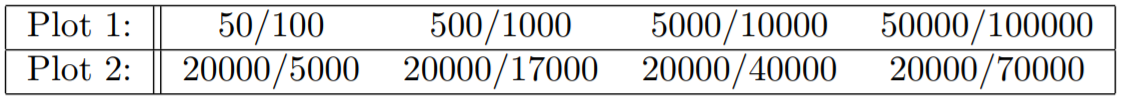
\includegraphics[width=0.7\linewidth]{tabledata}
	\caption{}
	\label{fig:tabledata}
\end{figure}

	The data in the figure \ref{fig:tabledata}, corresponds with figure \ref{fig:plot-1} (plot 1) and figure \ref{fig:plot-2} (plot 2). In figure \ref{fig:plot-1} we can observe that the ratio node/edges is equal among all plots. We have seen in the lectures that the larger is the graph, the more the probability that a random node has a link to \textit{k} other nodes is Poisson distributed. In the second plot, we keep the same number of nodes but increase the number of edges. This has the effect to increase the mean of the Poisson distribution. We can easily observe the orange, red, brown and grey bell curves sliding to the right as the number of edges increases. \\
	
	
	We fill the shorter distributions with zeros because Poisson distributions tend to zero and we assume the missing values (\textit{P(k)}) at the end of our tables, so for large \textit{k's}, will tend to zero. \\
	
	
	The ranges of the discrete distributions we obtain cannot be deterministic because we generate our graphs randomly. So the max degree of the distribution is random. 
	 


	
\begin{figure}[H]
	\centering
	\includegraphics[width=0.9\linewidth]{"../Scripts/Plot 1"}
	\caption{}
	\label{fig:plot-1}
\end{figure}


\begin{figure}[H]
	\centering
	\includegraphics[width=0.9\linewidth]{"../Scripts/Plot 2"}
	\caption{}
	\label{fig:plot-2}
\end{figure}






\end{enumerate}
\end{document}